\documentclass[twoside]{book}

% Packages required by doxygen
\usepackage{fixltx2e}
\usepackage{calc}
\usepackage{doxygen}
\usepackage[export]{adjustbox} % also loads graphicx
\usepackage{graphicx}
\usepackage[utf8]{inputenc}
\usepackage{makeidx}
\usepackage{multicol}
\usepackage{multirow}
\PassOptionsToPackage{warn}{textcomp}
\usepackage{textcomp}
\usepackage[nointegrals]{wasysym}
\usepackage[table]{xcolor}

% NLS support packages
Portuguese
% Font selection
\usepackage[T1]{fontenc}
\usepackage[scaled=.90]{helvet}
\usepackage{courier}
\usepackage{amssymb}
\usepackage{sectsty}
\renewcommand{\familydefault}{\sfdefault}
\allsectionsfont{%
  \fontseries{bc}\selectfont%
  \color{darkgray}%
}
\renewcommand{\DoxyLabelFont}{%
  \fontseries{bc}\selectfont%
  \color{darkgray}%
}
\newcommand{\+}{\discretionary{\mbox{\scriptsize$\hookleftarrow$}}{}{}}

% Page & text layout
\usepackage{geometry}
\geometry{%
  a4paper,%
  top=2.5cm,%
  bottom=2.5cm,%
  left=2.5cm,%
  right=2.5cm%
}
\tolerance=750
\hfuzz=15pt
\hbadness=750
\setlength{\emergencystretch}{15pt}
\setlength{\parindent}{0cm}
\setlength{\parskip}{3ex plus 2ex minus 2ex}
\makeatletter
\renewcommand{\paragraph}{%
  \@startsection{paragraph}{4}{0ex}{-1.0ex}{1.0ex}{%
    \normalfont\normalsize\bfseries\SS@parafont%
  }%
}
\renewcommand{\subparagraph}{%
  \@startsection{subparagraph}{5}{0ex}{-1.0ex}{1.0ex}{%
    \normalfont\normalsize\bfseries\SS@subparafont%
  }%
}
\makeatother

% Headers & footers
\usepackage{fancyhdr}
\pagestyle{fancyplain}
\fancyhead[LE]{\fancyplain{}{\bfseries\thepage}}
\fancyhead[CE]{\fancyplain{}{}}
\fancyhead[RE]{\fancyplain{}{\bfseries\leftmark}}
\fancyhead[LO]{\fancyplain{}{\bfseries\rightmark}}
\fancyhead[CO]{\fancyplain{}{}}
\fancyhead[RO]{\fancyplain{}{\bfseries\thepage}}
\fancyfoot[LE]{\fancyplain{}{}}
\fancyfoot[CE]{\fancyplain{}{}}
\fancyfoot[RE]{\fancyplain{}{\bfseries\scriptsize Gerado por Doxygen }}
\fancyfoot[LO]{\fancyplain{}{\bfseries\scriptsize Gerado por Doxygen }}
\fancyfoot[CO]{\fancyplain{}{}}
\fancyfoot[RO]{\fancyplain{}{}}
\renewcommand{\footrulewidth}{0.4pt}
\renewcommand{\chaptermark}[1]{%
  \markboth{#1}{}%
}
\renewcommand{\sectionmark}[1]{%
  \markright{\thesection\ #1}%
}

% Indices & bibliography
\usepackage{natbib}
\usepackage[titles]{tocloft}
\setcounter{tocdepth}{3}
\setcounter{secnumdepth}{5}
\makeindex

% Hyperlinks (required, but should be loaded last)
\usepackage{ifpdf}
\ifpdf
  \usepackage[pdftex,pagebackref=true]{hyperref}
\else
  \usepackage[ps2pdf,pagebackref=true]{hyperref}
\fi
\hypersetup{%
  colorlinks=true,%
  linkcolor=blue,%
  citecolor=blue,%
  unicode%
}

% Custom commands
\newcommand{\clearemptydoublepage}{%
  \newpage{\pagestyle{empty}\cleardoublepage}%
}

\usepackage{caption}
\captionsetup{labelsep=space,justification=centering,font={bf},singlelinecheck=off,skip=4pt,position=top}

%===== C O N T E N T S =====

\begin{document}

% Titlepage & ToC
\hypersetup{pageanchor=false,
             bookmarksnumbered=true,
             pdfencoding=unicode
            }
\pagenumbering{alph}
\begin{titlepage}
\vspace*{7cm}
\begin{center}%
{\Large Classes\+Abstratas \\[1ex]\large 1.\+0 }\\
\vspace*{1cm}
{\large Gerado por Doxygen 1.8.13}\\
\end{center}
\end{titlepage}
\clearemptydoublepage
\pagenumbering{roman}
\tableofcontents
\clearemptydoublepage
\pagenumbering{arabic}
\hypersetup{pageanchor=true}

%--- Begin generated contents ---
\chapter{Índice da hierarquia}
\section{Hierarquia de classes}
Esta lista de heranças está organizada, dentro do possível, por ordem alfabética\+:\begin{DoxyCompactList}
\item \contentsline{section}{Figura\+Geometrica}{\pageref{class_figura_geometrica}}{}
\begin{DoxyCompactList}
\item \contentsline{section}{Circulo}{\pageref{class_circulo}}{}
\item \contentsline{section}{Reta}{\pageref{class_reta}}{}
\item \contentsline{section}{Retangulo}{\pageref{class_retangulo}}{}
\end{DoxyCompactList}
\item \contentsline{section}{Screen}{\pageref{class_screen}}{}
\end{DoxyCompactList}

\chapter{Índice dos componentes}
\section{Lista de componentes}
Lista de classes, estruturas, uniões e interfaces com uma breve descrição\+:\begin{DoxyCompactList}
\item\contentsline{section}{\hyperlink{class_circulo}{Circulo} }{\pageref{class_circulo}}{}
\item\contentsline{section}{\hyperlink{class_figura_geometrica}{Figura\+Geometrica} }{\pageref{class_figura_geometrica}}{}
\item\contentsline{section}{\hyperlink{class_reta}{Reta} }{\pageref{class_reta}}{}
\item\contentsline{section}{\hyperlink{class_retangulo}{Retangulo} }{\pageref{class_retangulo}}{}
\item\contentsline{section}{\hyperlink{class_screen}{Screen} }{\pageref{class_screen}}{}
\end{DoxyCompactList}

\chapter{Índice dos ficheiros}
\section{Lista de ficheiros}
Lista de todos os ficheiros com uma breve descrição\+:\begin{DoxyCompactList}
\item\contentsline{section}{\hyperlink{circulo_8cpp}{circulo.\+cpp} }{\pageref{circulo_8cpp}}{}
\item\contentsline{section}{\hyperlink{circulo_8h}{circulo.\+h} }{\pageref{circulo_8h}}{}
\item\contentsline{section}{\hyperlink{figurageometrica_8cpp}{figurageometrica.\+cpp} }{\pageref{figurageometrica_8cpp}}{}
\item\contentsline{section}{\hyperlink{figurageometrica_8h}{figurageometrica.\+h} }{\pageref{figurageometrica_8h}}{}
\item\contentsline{section}{\hyperlink{main_8cpp}{main.\+cpp} }{\pageref{main_8cpp}}{}
\item\contentsline{section}{\hyperlink{reta_8cpp}{reta.\+cpp} }{\pageref{reta_8cpp}}{}
\item\contentsline{section}{\hyperlink{reta_8h}{reta.\+h} }{\pageref{reta_8h}}{}
\item\contentsline{section}{\hyperlink{retangulo_8cpp}{retangulo.\+cpp} }{\pageref{retangulo_8cpp}}{}
\item\contentsline{section}{\hyperlink{retangulo_8h}{retangulo.\+h} }{\pageref{retangulo_8h}}{}
\item\contentsline{section}{\hyperlink{screen_8cpp}{screen.\+cpp} }{\pageref{screen_8cpp}}{}
\item\contentsline{section}{\hyperlink{screen_8h}{screen.\+h} }{\pageref{screen_8h}}{}
\end{DoxyCompactList}

\chapter{Documentação da classe}
\hypertarget{class_circulo}{}\section{Referência à classe Circulo}
\label{class_circulo}\index{Circulo@{Circulo}}


{\ttfamily \#include $<$circulo.\+h$>$}

Diagrama de heranças da classe Circulo\begin{figure}[H]
\begin{center}
\leavevmode
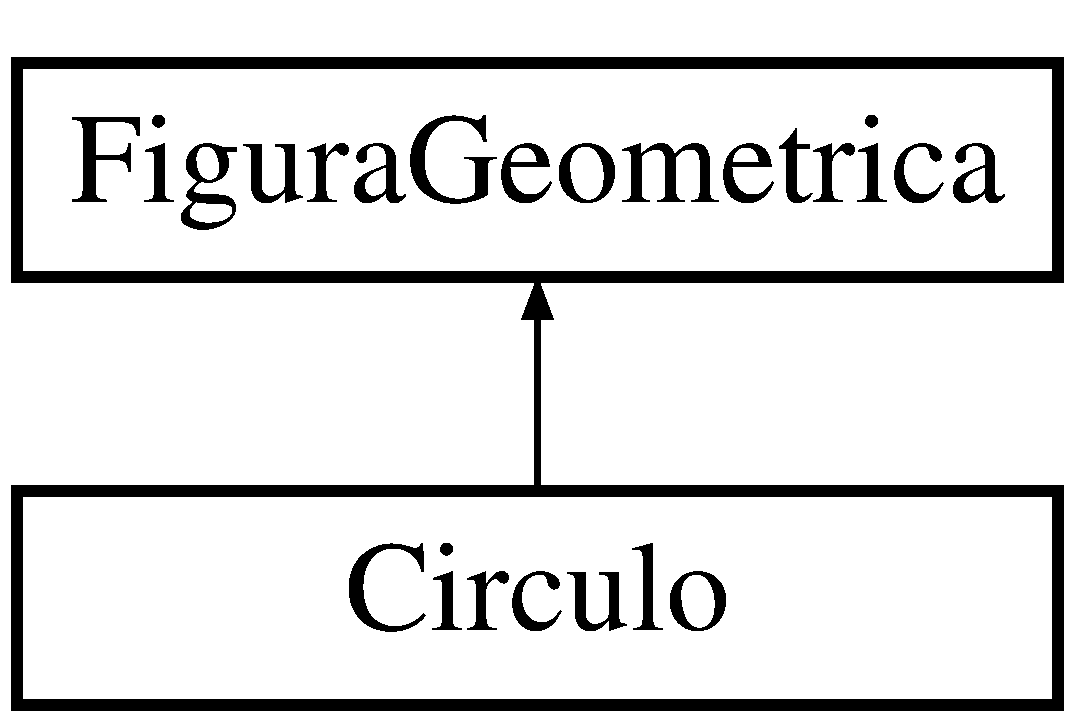
\includegraphics[height=2.000000cm]{class_circulo}
\end{center}
\end{figure}
\subsection*{Membros públicos}
\begin{DoxyCompactItemize}
\item 
\hyperlink{class_circulo_ad6da9864f1c91e281698e33aa3d18d6a}{Circulo} (int \+\_\+x0=0, int \+\_\+y0=0, int \+\_\+raio=1, int \+\_\+fillmode=1, char \+\_\+brush=\textquotesingle{} $\ast$\textquotesingle{})
\begin{DoxyCompactList}\small\item\em circulo é um contrutor para \hyperlink{class_circulo}{Circulo} em que têm-\/se como parâmeto, o ponto no centro do circulo, raio, a opção de preencher ou não o circulo e brush. \end{DoxyCompactList}\item 
void \hyperlink{class_circulo_a593787d6e0618c2eded23e8839e7bea6}{draw} (\hyperlink{class_screen}{Screen} \&t)
\begin{DoxyCompactList}\small\item\em draw é a função advinda da Classe \hyperlink{class_figura_geometrica}{Figura\+Geometrica} e é implementada no intuito de desenhar sobre a tela um círculo , neste caso. \end{DoxyCompactList}\end{DoxyCompactItemize}


\subsection{Documentação dos Construtores \& Destrutor}
\mbox{\Hypertarget{class_circulo_ad6da9864f1c91e281698e33aa3d18d6a}\label{class_circulo_ad6da9864f1c91e281698e33aa3d18d6a}} 
\index{Circulo@{Circulo}!Circulo@{Circulo}}
\index{Circulo@{Circulo}!Circulo@{Circulo}}
\subsubsection{\texorpdfstring{Circulo()}{Circulo()}}
{\footnotesize\ttfamily Circulo\+::\+Circulo (\begin{DoxyParamCaption}\item[{int}]{\+\_\+x0 = {\ttfamily 0},  }\item[{int}]{\+\_\+y0 = {\ttfamily 0},  }\item[{int}]{\+\_\+raio = {\ttfamily 1},  }\item[{int}]{\+\_\+fillmode = {\ttfamily 1},  }\item[{char}]{\+\_\+brush = {\ttfamily \textquotesingle{}$\ast$\textquotesingle{}} }\end{DoxyParamCaption})}



circulo é um contrutor para \hyperlink{class_circulo}{Circulo} em que têm-\/se como parâmeto, o ponto no centro do circulo, raio, a opção de preencher ou não o circulo e brush. 


\begin{DoxyParams}{Parâmetros}
{\em \+\_\+x0,x} & do ponto que centraliza o circulo \\
\hline
{\em \+\_\+y0,y} & do ponto que centraliza o circulo \\
\hline
{\em \+\_\+raio} & é o raio do circulo \\
\hline
{\em \+\_\+fillmode} & é a variavel que define se será ou não preenchido o circulo \\
\hline
{\em brush} & é o pincel \\
\hline
\end{DoxyParams}

\begin{DoxyCode}
4 \{
5     x0 = \_x0;
6     y0 = \_y0;
7     raio = \_raio;
8     fillmode = \_fillmode;
9     brush = \_brush;
10 
11 \}
\end{DoxyCode}


\subsection{Documentação dos métodos}
\mbox{\Hypertarget{class_circulo_a593787d6e0618c2eded23e8839e7bea6}\label{class_circulo_a593787d6e0618c2eded23e8839e7bea6}} 
\index{Circulo@{Circulo}!draw@{draw}}
\index{draw@{draw}!Circulo@{Circulo}}
\subsubsection{\texorpdfstring{draw()}{draw()}}
{\footnotesize\ttfamily void Circulo\+::draw (\begin{DoxyParamCaption}\item[{\hyperlink{class_screen}{Screen} \&}]{t }\end{DoxyParamCaption})\hspace{0.3cm}{\ttfamily [virtual]}}



draw é a função advinda da Classe \hyperlink{class_figura_geometrica}{Figura\+Geometrica} e é implementada no intuito de desenhar sobre a tela um círculo , neste caso. 


\begin{DoxyParams}{Parâmetros}
{\em t} & \\
\hline
\end{DoxyParams}


Implementa \hyperlink{class_figura_geometrica_a06404670d06d28d12f5f386901186925}{Figura\+Geometrica}.


\begin{DoxyCode}
13                            \{
14     t.\hyperlink{class_screen_aebc4eb6cb5acf15a0f04c1494622ab23}{setBrush}(brush);
15     \textcolor{keywordtype}{int} x = 0;
16     \textcolor{keywordtype}{int} y = raio;
17     \textcolor{keywordtype}{int} d = 1 - raio;
18     \textcolor{keywordflow}{while}(y > x)\{
19         \textcolor{comment}{//Desenha os pontos no 2 octante e nos octantes restantes}
20         t.\hyperlink{class_screen_ae6bea81c57a22d226507c3c26fa95ee0}{setPixel}(x0 + x, y0 + y);
21         t.\hyperlink{class_screen_ae6bea81c57a22d226507c3c26fa95ee0}{setPixel}(x0 + y, y0 + x);
22         t.\hyperlink{class_screen_ae6bea81c57a22d226507c3c26fa95ee0}{setPixel}(x0 - y, y0 + x);
23         t.\hyperlink{class_screen_ae6bea81c57a22d226507c3c26fa95ee0}{setPixel}(x0 - x, y0 + y);
24         t.\hyperlink{class_screen_ae6bea81c57a22d226507c3c26fa95ee0}{setPixel}(x0 - x, y0 - y);
25         t.\hyperlink{class_screen_ae6bea81c57a22d226507c3c26fa95ee0}{setPixel}(x0 - y, y0 - x);
26         t.\hyperlink{class_screen_ae6bea81c57a22d226507c3c26fa95ee0}{setPixel}(x0 + y, y0 - x);
27         t.\hyperlink{class_screen_ae6bea81c57a22d226507c3c26fa95ee0}{setPixel}(x0 + x, y0 - y);
28 
29         \textcolor{comment}{//Verifica se o circulo é preenchido e o desenha totalmente preenchido}
30         \textcolor{keywordflow}{if}(fillmode == 1)\{
31             \textcolor{keywordflow}{for} (\textcolor{keywordtype}{int} i = x0 - x; i <= x0 + x; i++)
32             \{
33                 t.\hyperlink{class_screen_ae6bea81c57a22d226507c3c26fa95ee0}{setPixel}(i, y0 + y);
34                 t.\hyperlink{class_screen_ae6bea81c57a22d226507c3c26fa95ee0}{setPixel}(i, y0 - y);
35             \}
36             \textcolor{keywordflow}{for} (\textcolor{keywordtype}{int} i = x0 - y; i <= x0 + y; i++)
37             \{
38                 t.\hyperlink{class_screen_ae6bea81c57a22d226507c3c26fa95ee0}{setPixel}(i, y0 + x);
39                 t.\hyperlink{class_screen_ae6bea81c57a22d226507c3c26fa95ee0}{setPixel}(i, y0 - x);
40             \}
41         \}
42         \textcolor{keywordflow}{if}(d < 0)\{
43             d = d + 2*x + 3;
44             x = x + 1;
45         \}
46         \textcolor{keywordflow}{else}\{
47             d = d + 2*(x-y) + 5;
48             x = x + 1;
49             y = y - 1;
50         \}
51     \}
52 \}
\end{DoxyCode}


A documentação para esta classe foi gerada a partir dos seguintes ficheiros\+:\begin{DoxyCompactItemize}
\item 
\hyperlink{circulo_8h}{circulo.\+h}\item 
\hyperlink{circulo_8cpp}{circulo.\+cpp}\end{DoxyCompactItemize}

\hypertarget{class_figura_geometrica}{}\section{Referência à classe Figura\+Geometrica}
\label{class_figura_geometrica}\index{Figura\+Geometrica@{Figura\+Geometrica}}


{\ttfamily \#include $<$figurageometrica.\+h$>$}

Diagrama de heranças da classe Figura\+Geometrica\begin{figure}[H]
\begin{center}
\leavevmode
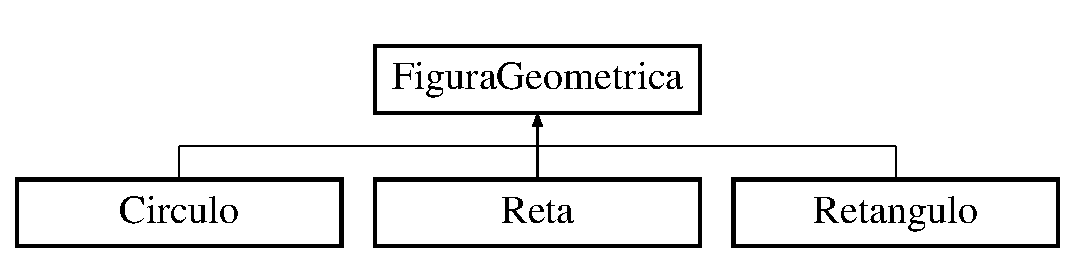
\includegraphics[height=2.000000cm]{class_figura_geometrica}
\end{center}
\end{figure}
\subsection*{Membros públicos}
\begin{DoxyCompactItemize}
\item 
\hyperlink{class_figura_geometrica_a81d7c7efaea511e60a15f5a363138dd9}{Figura\+Geometrica} ()
\item 
virtual void \hyperlink{class_figura_geometrica_a06404670d06d28d12f5f386901186925}{draw} (\hyperlink{class_screen}{Screen} \&t)=0
\begin{DoxyCompactList}\small\item\em draw é um método do tipo virtual; e, se todos os métodos da classe forem virtual, então pode-\/se dizer que a classe é abstrata pura. \end{DoxyCompactList}\end{DoxyCompactItemize}


\subsection{Documentação dos Construtores \& Destrutor}
\mbox{\Hypertarget{class_figura_geometrica_a81d7c7efaea511e60a15f5a363138dd9}\label{class_figura_geometrica_a81d7c7efaea511e60a15f5a363138dd9}} 
\index{Figura\+Geometrica@{Figura\+Geometrica}!Figura\+Geometrica@{Figura\+Geometrica}}
\index{Figura\+Geometrica@{Figura\+Geometrica}!Figura\+Geometrica@{Figura\+Geometrica}}
\subsubsection{\texorpdfstring{Figura\+Geometrica()}{FiguraGeometrica()}}
{\footnotesize\ttfamily Figura\+Geometrica\+::\+Figura\+Geometrica (\begin{DoxyParamCaption}{ }\end{DoxyParamCaption})}


\begin{DoxyCode}
5 \{
6 \}
\end{DoxyCode}


\subsection{Documentação dos métodos}
\mbox{\Hypertarget{class_figura_geometrica_a06404670d06d28d12f5f386901186925}\label{class_figura_geometrica_a06404670d06d28d12f5f386901186925}} 
\index{Figura\+Geometrica@{Figura\+Geometrica}!draw@{draw}}
\index{draw@{draw}!Figura\+Geometrica@{Figura\+Geometrica}}
\subsubsection{\texorpdfstring{draw()}{draw()}}
{\footnotesize\ttfamily void Figura\+Geometrica\+::draw (\begin{DoxyParamCaption}\item[{\hyperlink{class_screen}{Screen} \&}]{t }\end{DoxyParamCaption})\hspace{0.3cm}{\ttfamily [pure virtual]}}



draw é um método do tipo virtual; e, se todos os métodos da classe forem virtual, então pode-\/se dizer que a classe é abstrata pura. 


\begin{DoxyParams}{Parâmetros}
{\em t} & \\
\hline
\end{DoxyParams}


Implementado em \hyperlink{class_circulo_a593787d6e0618c2eded23e8839e7bea6}{Circulo}, \hyperlink{class_reta_ac2e9805183cd474b62bffd8b032cd780}{Reta} e \hyperlink{class_retangulo_ac088dd6d3f4f3d3f80363a868c2e74f1}{Retangulo}.


\begin{DoxyCode}
8                                      \{
9 
10 \}
\end{DoxyCode}


A documentação para esta classe foi gerada a partir dos seguintes ficheiros\+:\begin{DoxyCompactItemize}
\item 
\hyperlink{figurageometrica_8h}{figurageometrica.\+h}\item 
\hyperlink{figurageometrica_8cpp}{figurageometrica.\+cpp}\end{DoxyCompactItemize}

\hypertarget{class_reta}{}\section{Referência à classe Reta}
\label{class_reta}\index{Reta@{Reta}}


{\ttfamily \#include $<$reta.\+h$>$}

Diagrama de heranças da classe Reta\begin{figure}[H]
\begin{center}
\leavevmode
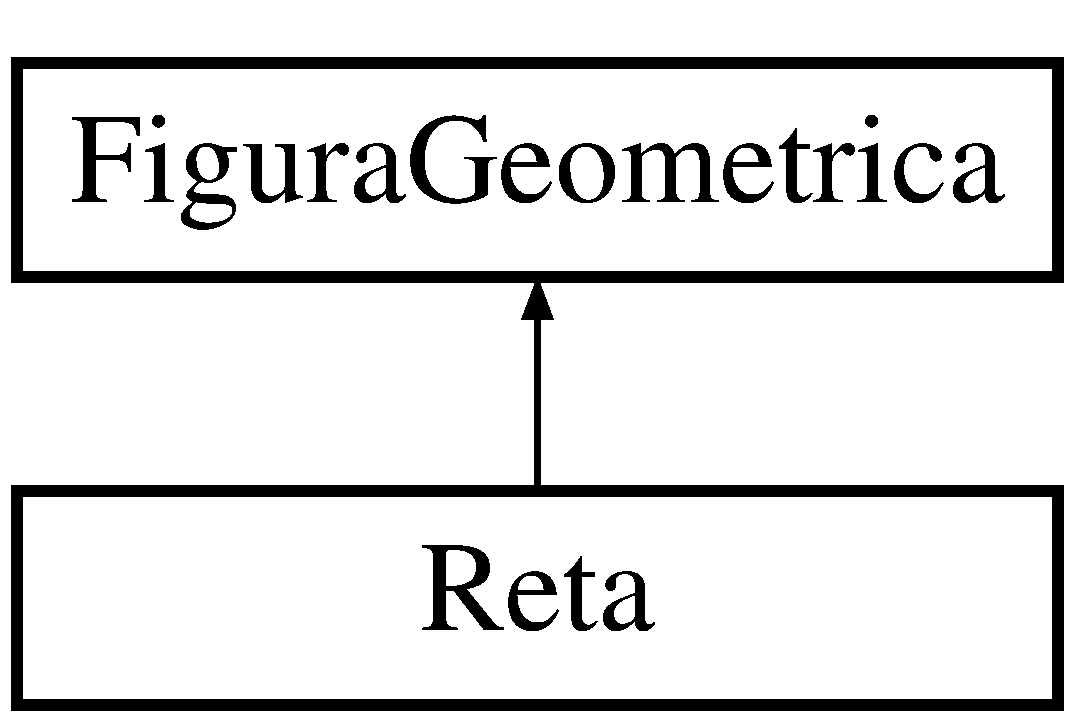
\includegraphics[height=2.000000cm]{class_reta}
\end{center}
\end{figure}
\subsection*{Membros públicos}
\begin{DoxyCompactItemize}
\item 
\hyperlink{class_reta_a5b0e120cd00f7bd931c30a62ead00d13}{Reta} (int \+\_\+pxi, int \+\_\+pyi, int \+\_\+pxf, int \+\_\+pyf, char \+\_\+brush)
\begin{DoxyCompactList}\small\item\em \hyperlink{class_reta}{Reta} é um construtor -\/ onde inicializa o ponto inicial e o final da reta. \end{DoxyCompactList}\item 
void \hyperlink{class_reta_ac2e9805183cd474b62bffd8b032cd780}{draw} (\hyperlink{class_screen}{Screen} \&t)
\begin{DoxyCompactList}\small\item\em draw é uma função que aproxima uma reta por meio do algoritmo de Bresenham. \end{DoxyCompactList}\item 
int \hyperlink{class_reta_a0890517655f27827a827c88850f8984e}{Sinal} (int x)
\begin{DoxyCompactList}\small\item\em Sinal é uma função auxiliar para alternar entre linhas de rasterização. \end{DoxyCompactList}\end{DoxyCompactItemize}


\subsection{Documentação dos Construtores \& Destrutor}
\mbox{\Hypertarget{class_reta_a5b0e120cd00f7bd931c30a62ead00d13}\label{class_reta_a5b0e120cd00f7bd931c30a62ead00d13}} 
\index{Reta@{Reta}!Reta@{Reta}}
\index{Reta@{Reta}!Reta@{Reta}}
\subsubsection{\texorpdfstring{Reta()}{Reta()}}
{\footnotesize\ttfamily Reta\+::\+Reta (\begin{DoxyParamCaption}\item[{int}]{\+\_\+pxi,  }\item[{int}]{\+\_\+pyi,  }\item[{int}]{\+\_\+pxf,  }\item[{int}]{\+\_\+pyf,  }\item[{char}]{\+\_\+brush }\end{DoxyParamCaption})}



\hyperlink{class_reta}{Reta} é um construtor -\/ onde inicializa o ponto inicial e o final da reta. 


\begin{DoxyParams}{Parâmetros}
{\em \+\_\+pxi} & é a coordenada x do ponto inicial \\
\hline
{\em \+\_\+pyi} & é a coordenada y do ponto inicial \\
\hline
{\em \+\_\+pxf} & é a coordenada x do ponto final \\
\hline
{\em \+\_\+pyf} & é a coordenada y do ponto final \\
\hline
\end{DoxyParams}

\begin{DoxyCode}
9 \{
10     pxi = \_pxi;
11     pyi = \_pyi;
12     pxf = \_pxf;
13     pyf = \_pyf;
14     brush = \_brush;
15 \}
\end{DoxyCode}


\subsection{Documentação dos métodos}
\mbox{\Hypertarget{class_reta_ac2e9805183cd474b62bffd8b032cd780}\label{class_reta_ac2e9805183cd474b62bffd8b032cd780}} 
\index{Reta@{Reta}!draw@{draw}}
\index{draw@{draw}!Reta@{Reta}}
\subsubsection{\texorpdfstring{draw()}{draw()}}
{\footnotesize\ttfamily void Reta\+::draw (\begin{DoxyParamCaption}\item[{\hyperlink{class_screen}{Screen} \&}]{t }\end{DoxyParamCaption})\hspace{0.3cm}{\ttfamily [virtual]}}



draw é uma função que aproxima uma reta por meio do algoritmo de Bresenham. 


\begin{DoxyParams}{Parâmetros}
{\em t} & é uma variável do tipo \hyperlink{class_screen}{Screen} que recebe o desenho da reta. \\
\hline
\end{DoxyParams}


Implementa \hyperlink{class_figura_geometrica_a06404670d06d28d12f5f386901186925}{Figura\+Geometrica}.


\begin{DoxyCode}
18 \{
19     \textcolor{comment}{//Altera o caracter de desenho}
20     t.\hyperlink{class_screen_aebc4eb6cb5acf15a0f04c1494622ab23}{setBrush}(brush);
21     \textcolor{keywordtype}{int} x = pxi;
22     \textcolor{keywordtype}{int} y = pyi;
23     \textcolor{keywordtype}{int} Troca;
24     \textcolor{keywordtype}{int} Delta\_x = abs(pxf - pxi);
25     \textcolor{keywordtype}{int} Delta\_y = abs(pyf - pyi);
26     \textcolor{keywordtype}{int} s1 = \hyperlink{class_reta_a0890517655f27827a827c88850f8984e}{Sinal}(pxf - pxi);
27     \textcolor{keywordtype}{int} s2 = \hyperlink{class_reta_a0890517655f27827a827c88850f8984e}{Sinal}(pyf - pyi);
28 
29     \textcolor{keywordflow}{if}(Delta\_y > Delta\_x)\{
30         \textcolor{keywordtype}{int} Temp = Delta\_x;
31         Delta\_x = Delta\_y;
32         Delta\_y = Temp;
33         Troca = 1;
34     \} \textcolor{keywordflow}{else}\{
35         Troca = 0;
36     \}
37 
38     \textcolor{keywordtype}{int} new\_e = 2*Delta\_y - Delta\_x;
39     \textcolor{keywordflow}{for}(\textcolor{keywordtype}{int} i = 1; i <= Delta\_x; i++)\{
40         t.\hyperlink{class_screen_ae6bea81c57a22d226507c3c26fa95ee0}{setPixel}(x,y);
41         \textcolor{keywordflow}{while} (new\_e >= 0)\{
42             \textcolor{keywordflow}{if}(Troca == 1)\{
43                 \textcolor{comment}{//Muda para a proxima linha de rasterização}
44                 x = x + s1;
45             \} \textcolor{keywordflow}{else}\{
46                 y = y + s2;
47             \}
48             new\_e = new\_e - 2*Delta\_x;
49         \}
50 
51         \textcolor{comment}{//Permanece nesta linha de rasterização}
52         \textcolor{keywordflow}{if}(Troca == 1)\{
53             y = y + s2;
54         \} \textcolor{keywordflow}{else}\{
55             x = x + s1;
56         \}
57         new\_e = new\_e + 2*Delta\_y;
58     \}
59 \}
\end{DoxyCode}
\mbox{\Hypertarget{class_reta_a0890517655f27827a827c88850f8984e}\label{class_reta_a0890517655f27827a827c88850f8984e}} 
\index{Reta@{Reta}!Sinal@{Sinal}}
\index{Sinal@{Sinal}!Reta@{Reta}}
\subsubsection{\texorpdfstring{Sinal()}{Sinal()}}
{\footnotesize\ttfamily int Reta\+::\+Sinal (\begin{DoxyParamCaption}\item[{int}]{x }\end{DoxyParamCaption})}



Sinal é uma função auxiliar para alternar entre linhas de rasterização. 


\begin{DoxyParams}{Parâmetros}
{\em x} & é o parâmetro utilizado para determinar se o retorno da função será entre -\/1, 0 e 1 \\
\hline
\end{DoxyParams}
\begin{DoxyReturn}{Retorna}

\end{DoxyReturn}

\begin{DoxyCode}
62 \{
63     \textcolor{keywordflow}{if}(x < 0)\{ \textcolor{keywordflow}{return} -1; \}
64     \textcolor{keywordflow}{if}(x == 0)\{ \textcolor{keywordflow}{return} 0; \}
65     \textcolor{keywordflow}{return} 1;
66 \}
\end{DoxyCode}


A documentação para esta classe foi gerada a partir dos seguintes ficheiros\+:\begin{DoxyCompactItemize}
\item 
\hyperlink{reta_8h}{reta.\+h}\item 
\hyperlink{reta_8cpp}{reta.\+cpp}\end{DoxyCompactItemize}

\hypertarget{class_retangulo}{}\section{Referência à classe Retangulo}
\label{class_retangulo}\index{Retangulo@{Retangulo}}


{\ttfamily \#include $<$retangulo.\+h$>$}

Diagrama de heranças da classe Retangulo\begin{figure}[H]
\begin{center}
\leavevmode
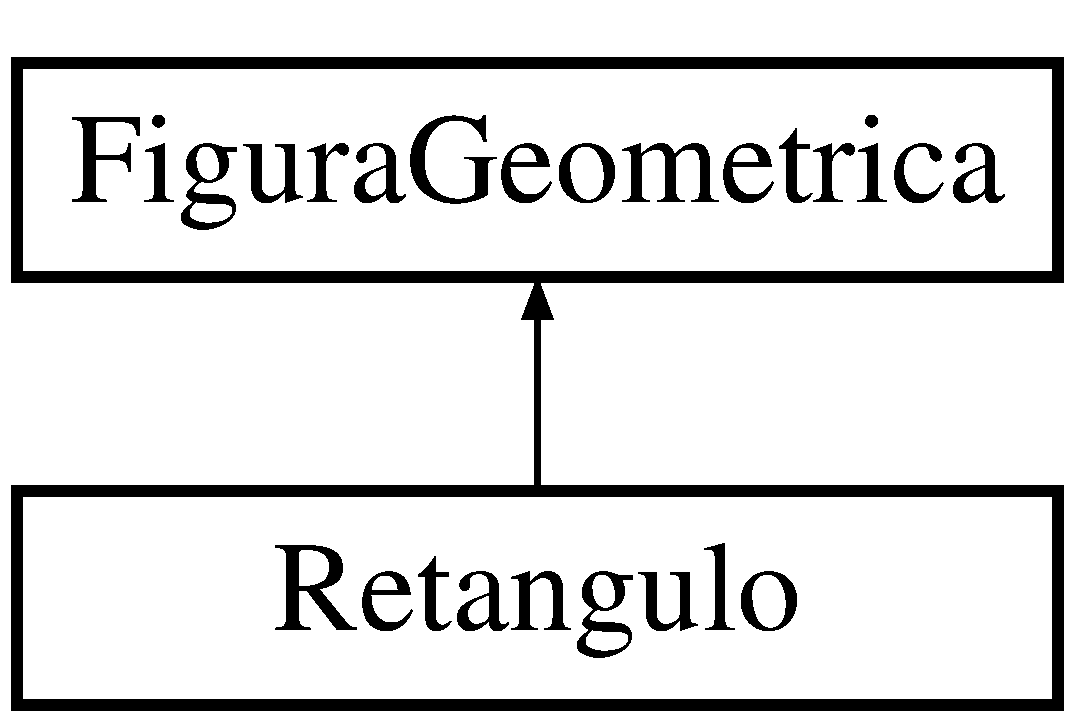
\includegraphics[height=2.000000cm]{class_retangulo}
\end{center}
\end{figure}
\subsection*{Membros públicos}
\begin{DoxyCompactItemize}
\item 
\hyperlink{class_retangulo_a93eeef9b155c5bb9f19d3c8d4013b43c}{Retangulo} (int \+\_\+x=0, int \+\_\+y=0, int \+\_\+l=0, int \+\_\+h=0, int \+\_\+fillmode=1, char \+\_\+brush=\textquotesingle{} $\ast$\textquotesingle{})
\begin{DoxyCompactList}\small\item\em Construtor do retângulo, onde recebe as coordenadas do ponto superior esquerdo e inicializa as variaveis privadas com os valores armazenados. \end{DoxyCompactList}\item 
void \hyperlink{class_retangulo_ac088dd6d3f4f3d3f80363a868c2e74f1}{draw} (\hyperlink{class_screen}{Screen} \&t)
\begin{DoxyCompactList}\small\item\em draw é um método do tipo virtual; e, se todos os métodos da classe forem virtual, então pode-\/se dizer que a classe é abstrata pura. \end{DoxyCompactList}\end{DoxyCompactItemize}


\subsection{Documentação dos Construtores \& Destrutor}
\mbox{\Hypertarget{class_retangulo_a93eeef9b155c5bb9f19d3c8d4013b43c}\label{class_retangulo_a93eeef9b155c5bb9f19d3c8d4013b43c}} 
\index{Retangulo@{Retangulo}!Retangulo@{Retangulo}}
\index{Retangulo@{Retangulo}!Retangulo@{Retangulo}}
\subsubsection{\texorpdfstring{Retangulo()}{Retangulo()}}
{\footnotesize\ttfamily Retangulo\+::\+Retangulo (\begin{DoxyParamCaption}\item[{int}]{\+\_\+x = {\ttfamily 0},  }\item[{int}]{\+\_\+y = {\ttfamily 0},  }\item[{int}]{\+\_\+l = {\ttfamily 0},  }\item[{int}]{\+\_\+h = {\ttfamily 0},  }\item[{int}]{\+\_\+fillmode = {\ttfamily 1},  }\item[{char}]{\+\_\+brush = {\ttfamily \textquotesingle{}$\ast$\textquotesingle{}} }\end{DoxyParamCaption})}



Construtor do retângulo, onde recebe as coordenadas do ponto superior esquerdo e inicializa as variaveis privadas com os valores armazenados. 


\begin{DoxyParams}{Parâmetros}
{\em \+\_\+x} & é a coordenada x do ponto superior esquerdo \\
\hline
{\em \+\_\+y} & é a coordenada y do ponto superior esquerdo \\
\hline
{\em \+\_\+l} & é a largura do retangulo \\
\hline
{\em \+\_\+h} & é a altura do retangulo \\
\hline
\end{DoxyParams}

\begin{DoxyCode}
4                                                                               \{
5     x= \_x;
6     y= \_y;
7     l= \_l;
8     h= \_h;
9     fillmode=\_fillmode;
10     brush=\_brush;
11 \}
\end{DoxyCode}


\subsection{Documentação dos métodos}
\mbox{\Hypertarget{class_retangulo_ac088dd6d3f4f3d3f80363a868c2e74f1}\label{class_retangulo_ac088dd6d3f4f3d3f80363a868c2e74f1}} 
\index{Retangulo@{Retangulo}!draw@{draw}}
\index{draw@{draw}!Retangulo@{Retangulo}}
\subsubsection{\texorpdfstring{draw()}{draw()}}
{\footnotesize\ttfamily void Retangulo\+::draw (\begin{DoxyParamCaption}\item[{\hyperlink{class_screen}{Screen} \&}]{t }\end{DoxyParamCaption})\hspace{0.3cm}{\ttfamily [virtual]}}



draw é um método do tipo virtual; e, se todos os métodos da classe forem virtual, então pode-\/se dizer que a classe é abstrata pura. 


\begin{DoxyParams}{Parâmetros}
{\em t} & \\
\hline
\end{DoxyParams}


Implementa \hyperlink{class_figura_geometrica_a06404670d06d28d12f5f386901186925}{Figura\+Geometrica}.


\begin{DoxyCode}
13                              \{
14     t.\hyperlink{class_screen_aebc4eb6cb5acf15a0f04c1494622ab23}{setBrush}(brush);
15 
16     \textcolor{keywordflow}{if}(fillmode>0)\{
17         \textcolor{keywordflow}{for}(\textcolor{keywordtype}{int} i=x; i<(x+l);i++)\{
18             \textcolor{keywordflow}{for}(\textcolor{keywordtype}{int} j=y;j<(y+h);j++)\{
19                 t.\hyperlink{class_screen_ae6bea81c57a22d226507c3c26fa95ee0}{setPixel}(i,j);
20             \}
21         \}
22     \}
23     \textcolor{keywordflow}{else}\{
24         \textcolor{keywordflow}{for}(\textcolor{keywordtype}{int} i=x; i<(x+l);i++)\{
25             \textcolor{keywordflow}{for}(\textcolor{keywordtype}{int} j=y;j<(y+h);j++)\{
26                 \textcolor{keywordflow}{if}(((i == x || i==x+l-1) || (j ==y || j==y+h-1)))\{
27                 t.\hyperlink{class_screen_ae6bea81c57a22d226507c3c26fa95ee0}{setPixel}(i,j);
28                 \}
29             \}
30         \}
31     \}
32 \}
\end{DoxyCode}


A documentação para esta classe foi gerada a partir dos seguintes ficheiros\+:\begin{DoxyCompactItemize}
\item 
\hyperlink{retangulo_8h}{retangulo.\+h}\item 
\hyperlink{retangulo_8cpp}{retangulo.\+cpp}\end{DoxyCompactItemize}

\hypertarget{class_screen}{}\section{Referência à classe Screen}
\label{class_screen}\index{Screen@{Screen}}


{\ttfamily \#include $<$screen.\+h$>$}

\subsection*{Membros públicos}
\begin{DoxyCompactItemize}
\item 
\hyperlink{class_screen_a6c21beca43d25854d8674445127ef2eb}{Screen} (int \+\_\+nlin, int \+\_\+ncol)
\begin{DoxyCompactList}\small\item\em \hyperlink{class_screen}{Screen} é o construtor da classe -\/ onde inicializa o número de linhas e de colunas da tela. \end{DoxyCompactList}\item 
void \hyperlink{class_screen_ae6bea81c57a22d226507c3c26fa95ee0}{set\+Pixel} (int x, int y)
\begin{DoxyCompactList}\small\item\em set\+Pixel desenha um pixel da matriz usando o caractere guardado em brush \end{DoxyCompactList}\item 
void \hyperlink{class_screen_a35e74266b2a04e37b354ceff7a5f1031}{clear} ()
\begin{DoxyCompactList}\small\item\em clear é um método da classe \hyperlink{class_screen}{Screen} que serve para limpar a tela. \end{DoxyCompactList}\item 
void \hyperlink{class_screen_a59f2c3f9e889b425940749e8f646db72}{set\+Screen} (int nl, int nc)
\begin{DoxyCompactList}\small\item\em set\+Screen utilizado para alterar as dimensões da tela \end{DoxyCompactList}\item 
void \hyperlink{class_screen_aebc4eb6cb5acf15a0f04c1494622ab23}{set\+Brush} (char \+\_\+brush)
\begin{DoxyCompactList}\small\item\em set\+Brush é um método da classe o qual muda o caractere a ser impresso na tela \end{DoxyCompactList}\end{DoxyCompactItemize}
\subsection*{Amigos}
\begin{DoxyCompactItemize}
\item 
ostream \& \hyperlink{class_screen_aab6a2880746bfe1b7964817cc8f0989e}{operator$<$$<$} (ostream \&os, \hyperlink{class_screen}{Screen} \&t)
\begin{DoxyCompactList}\small\item\em operator $<$$<$ \end{DoxyCompactList}\end{DoxyCompactItemize}


\subsection{Documentação dos Construtores \& Destrutor}
\mbox{\Hypertarget{class_screen_a6c21beca43d25854d8674445127ef2eb}\label{class_screen_a6c21beca43d25854d8674445127ef2eb}} 
\index{Screen@{Screen}!Screen@{Screen}}
\index{Screen@{Screen}!Screen@{Screen}}
\subsubsection{\texorpdfstring{Screen()}{Screen()}}
{\footnotesize\ttfamily Screen\+::\+Screen (\begin{DoxyParamCaption}\item[{int}]{\+\_\+nlin,  }\item[{int}]{\+\_\+ncol }\end{DoxyParamCaption})}



\hyperlink{class_screen}{Screen} é o construtor da classe -\/ onde inicializa o número de linhas e de colunas da tela. 


\begin{DoxyParams}{Parâmetros}
{\em \+\_\+nlin} & é o número de linhas \\
\hline
{\em \+\_\+ncol} & é o número de colunas \\
\hline
\end{DoxyParams}

\begin{DoxyCode}
8                                   \{
9     nlin = \_nlin;
10     ncol = \_ncol;
11     mat = vector<vector<char>>(nlin, vector<char>(ncol)); 
12     
13     brush = \textcolor{charliteral}{' '};
14     
15 \}
\end{DoxyCode}


\subsection{Documentação dos métodos}
\mbox{\Hypertarget{class_screen_a35e74266b2a04e37b354ceff7a5f1031}\label{class_screen_a35e74266b2a04e37b354ceff7a5f1031}} 
\index{Screen@{Screen}!clear@{clear}}
\index{clear@{clear}!Screen@{Screen}}
\subsubsection{\texorpdfstring{clear()}{clear()}}
{\footnotesize\ttfamily void Screen\+::clear (\begin{DoxyParamCaption}{ }\end{DoxyParamCaption})}



clear é um método da classe \hyperlink{class_screen}{Screen} que serve para limpar a tela. 


\begin{DoxyCode}
28                   \{
29     \textcolor{keywordflow}{for}(\textcolor{keywordtype}{int} i=0; i<nlin; i++)\{
30         \textcolor{keywordflow}{for}(\textcolor{keywordtype}{int} j=0; j<ncol; j++)\{
31             mat[i][j]= \textcolor{charliteral}{' '};
32         \}
33     \}
34 \}
\end{DoxyCode}
\mbox{\Hypertarget{class_screen_aebc4eb6cb5acf15a0f04c1494622ab23}\label{class_screen_aebc4eb6cb5acf15a0f04c1494622ab23}} 
\index{Screen@{Screen}!set\+Brush@{set\+Brush}}
\index{set\+Brush@{set\+Brush}!Screen@{Screen}}
\subsubsection{\texorpdfstring{set\+Brush()}{setBrush()}}
{\footnotesize\ttfamily void Screen\+::set\+Brush (\begin{DoxyParamCaption}\item[{char}]{\+\_\+brush }\end{DoxyParamCaption})}



set\+Brush é um método da classe o qual muda o caractere a ser impresso na tela 


\begin{DoxyParams}{Parâmetros}
{\em \+\_\+brush} & inicializa o novo caractere \\
\hline
\end{DoxyParams}

\begin{DoxyCode}
36                                 \{
37     brush = \_brush;
38 \}
\end{DoxyCode}
\mbox{\Hypertarget{class_screen_ae6bea81c57a22d226507c3c26fa95ee0}\label{class_screen_ae6bea81c57a22d226507c3c26fa95ee0}} 
\index{Screen@{Screen}!set\+Pixel@{set\+Pixel}}
\index{set\+Pixel@{set\+Pixel}!Screen@{Screen}}
\subsubsection{\texorpdfstring{set\+Pixel()}{setPixel()}}
{\footnotesize\ttfamily void Screen\+::set\+Pixel (\begin{DoxyParamCaption}\item[{int}]{x,  }\item[{int}]{y }\end{DoxyParamCaption})}



set\+Pixel desenha um pixel da matriz usando o caractere guardado em brush 


\begin{DoxyParams}{Parâmetros}
{\em x} & \\
\hline
{\em y} & \\
\hline
\end{DoxyParams}

\begin{DoxyCode}
17                                  \{
18     \textcolor{keywordflow}{if}((x>=0 && x<nlin) && (y>=0 && y<nlin)) mat[x][y]= brush;
19 \}
\end{DoxyCode}
\mbox{\Hypertarget{class_screen_a59f2c3f9e889b425940749e8f646db72}\label{class_screen_a59f2c3f9e889b425940749e8f646db72}} 
\index{Screen@{Screen}!set\+Screen@{set\+Screen}}
\index{set\+Screen@{set\+Screen}!Screen@{Screen}}
\subsubsection{\texorpdfstring{set\+Screen()}{setScreen()}}
{\footnotesize\ttfamily void Screen\+::set\+Screen (\begin{DoxyParamCaption}\item[{int}]{nl,  }\item[{int}]{nc }\end{DoxyParamCaption})}



set\+Screen utilizado para alterar as dimensões da tela 


\begin{DoxyParams}{Parâmetros}
{\em nl} & \\
\hline
{\em nc} & \\
\hline
\end{DoxyParams}

\begin{DoxyCode}
22 \{
23     nlin = nl;
24     ncol = nc;
25     mat = vector< vector<char> >(nlin, vector<char>(ncol,\textcolor{charliteral}{' '}));
26 \}
\end{DoxyCode}


\subsection{Documentação das classes amigas e funções relacionadas}
\mbox{\Hypertarget{class_screen_aab6a2880746bfe1b7964817cc8f0989e}\label{class_screen_aab6a2880746bfe1b7964817cc8f0989e}} 
\index{Screen@{Screen}!operator$<$$<$@{operator$<$$<$}}
\index{operator$<$$<$@{operator$<$$<$}!Screen@{Screen}}
\subsubsection{\texorpdfstring{operator$<$$<$}{operator<<}}
{\footnotesize\ttfamily ostream\& operator$<$$<$ (\begin{DoxyParamCaption}\item[{ostream \&}]{os,  }\item[{\hyperlink{class_screen}{Screen} \&}]{t }\end{DoxyParamCaption})\hspace{0.3cm}{\ttfamily [friend]}}



operator $<$$<$ 


\begin{DoxyParams}{Parâmetros}
{\em os} & \\
\hline
{\em t} & \\
\hline
\end{DoxyParams}
\begin{DoxyReturn}{Retorna}

\end{DoxyReturn}

\begin{DoxyCode}
40                                            \{
41     \textcolor{keywordflow}{for}(\textcolor{keywordtype}{int} i=0;i<t.nlin;i++)\{
42         \textcolor{keywordflow}{for}(\textcolor{keywordtype}{int} j=0; j<t.ncol; j++)\{
43             os<< t.mat[j][i] <<\textcolor{stringliteral}{" "};
44         \}
45         os<<endl;
46     \}
47 
48     \textcolor{keywordflow}{return} os;
49 \}
\end{DoxyCode}


A documentação para esta classe foi gerada a partir dos seguintes ficheiros\+:\begin{DoxyCompactItemize}
\item 
\hyperlink{screen_8h}{screen.\+h}\item 
\hyperlink{screen_8cpp}{screen.\+cpp}\end{DoxyCompactItemize}

\chapter{Documentação do ficheiro}
\hypertarget{circulo_8cpp}{}\section{Referência ao ficheiro circulo.\+cpp}
\label{circulo_8cpp}\index{circulo.\+cpp@{circulo.\+cpp}}
{\ttfamily \#include \char`\"{}circulo.\+h\char`\"{}}\newline

\hypertarget{circulo_8h}{}\section{Referência ao ficheiro circulo.\+h}
\label{circulo_8h}\index{circulo.\+h@{circulo.\+h}}
{\ttfamily \#include $<$iostream$>$}\newline
{\ttfamily \#include \char`\"{}figurageometrica.\+h\char`\"{}}\newline
\subsection*{Componentes}
\begin{DoxyCompactItemize}
\item 
class \hyperlink{class_circulo}{Circulo}
\end{DoxyCompactItemize}

\hypertarget{figurageometrica_8cpp}{}\section{Referência ao ficheiro figurageometrica.\+cpp}
\label{figurageometrica_8cpp}\index{figurageometrica.\+cpp@{figurageometrica.\+cpp}}
{\ttfamily \#include \char`\"{}figurageometrica.\+h\char`\"{}}\newline
{\ttfamily \#include \char`\"{}screen.\+h\char`\"{}}\newline

\hypertarget{figurageometrica_8h}{}\section{Referência ao ficheiro figurageometrica.\+h}
\label{figurageometrica_8h}\index{figurageometrica.\+h@{figurageometrica.\+h}}
{\ttfamily \#include \char`\"{}screen.\+h\char`\"{}}\newline
\subsection*{Componentes}
\begin{DoxyCompactItemize}
\item 
class \hyperlink{class_figura_geometrica}{Figura\+Geometrica}
\end{DoxyCompactItemize}

\hypertarget{main_8cpp}{}\section{Referência ao ficheiro main.\+cpp}
\label{main_8cpp}\index{main.\+cpp@{main.\+cpp}}
{\ttfamily \#include $<$iostream$>$}\newline
{\ttfamily \#include $<$fstream$>$}\newline
{\ttfamily \#include \char`\"{}figurageometrica.\+h\char`\"{}}\newline
{\ttfamily \#include \char`\"{}screen.\+h\char`\"{}}\newline
{\ttfamily \#include \char`\"{}retangulo.\+h\char`\"{}}\newline
{\ttfamily \#include \char`\"{}reta.\+h\char`\"{}}\newline
{\ttfamily \#include \char`\"{}circulo.\+h\char`\"{}}\newline
{\ttfamily \#include $<$string$>$}\newline
{\ttfamily \#include $<$sstream$>$}\newline
{\ttfamily \#include $<$list$>$}\newline
\subsection*{Funções}
\begin{DoxyCompactItemize}
\item 
int \hyperlink{main_8cpp_ae66f6b31b5ad750f1fe042a706a4e3d4}{main} ()
\end{DoxyCompactItemize}


\subsection{Documentação das funções}
\mbox{\Hypertarget{main_8cpp_ae66f6b31b5ad750f1fe042a706a4e3d4}\label{main_8cpp_ae66f6b31b5ad750f1fe042a706a4e3d4}} 
\index{main.\+cpp@{main.\+cpp}!main@{main}}
\index{main@{main}!main.\+cpp@{main.\+cpp}}
\subsubsection{\texorpdfstring{main()}{main()}}
{\footnotesize\ttfamily int main (\begin{DoxyParamCaption}{ }\end{DoxyParamCaption})}


\begin{DoxyCode}
15 \{
16     ifstream fin;
17     ofstream fout;
18     \hyperlink{class_screen}{Screen} t(50,50);
19     \textcolor{keywordtype}{string} s;
20     fin.open(\textcolor{stringliteral}{"/home/mneto/Documentos/Facul/Programação Avançada/Unidade II/projeto2/instrucoes.txt"});
21     \textcolor{keywordflow}{if}(!fin.is\_open())\{
22         cout << \textcolor{stringliteral}{"nao abriu arquivo\(\backslash\)n"};
23     \}
24     fout.open(\textcolor{stringliteral}{"/home/mneto/Documentos/Facul/Programação Avançada/Unidade II/projeto2/figura.txt"});
25     list <FiguraGeometrica*>::iterator fg;
26     list <FiguraGeometrica*> figuras;
27     \textcolor{keywordflow}{while}(fin.good())\{
28         getline(fin, s);
29         \textcolor{keywordflow}{if}(fin.good())\{
30             \textcolor{keywordtype}{string} cmd;
31             stringstream sstream(s);
32             sstream >> cmd;
33             \textcolor{keywordflow}{if}(cmd.compare(\textcolor{stringliteral}{"dim"})==0)\{
34                 \textcolor{keywordtype}{int} x, y;
35                 sstream >> x >> y;
36                 t.setScreen(x,y);
37             \}
38             \textcolor{keywordflow}{if}(cmd.compare(\textcolor{stringliteral}{"Reta"})==0)\{
39                 \textcolor{keywordtype}{int} pxi, pyi, pxf,pyf;
40                 \textcolor{keywordtype}{char} brush;
41                 sstream >> pxi >>pyi >> pxf >> pyf >> brush;
42                 figuras.push\_back(\textcolor{keyword}{new} \hyperlink{class_reta}{Reta}(pxi,pyi,pxf,pyf,brush));
43             \}
44             \textcolor{keywordflow}{if}(cmd.compare(\textcolor{stringliteral}{"Retangulo"})==0)\{
45                 \textcolor{keywordtype}{int} x,y,h,l;
46                 \textcolor{keywordtype}{int} fillmode;
47                 \textcolor{keywordtype}{char} brush;
48                 sstream >> x >> y >> l >> h >>fillmode >> brush;
49                 figuras.push\_back(\textcolor{keyword}{new} \hyperlink{class_retangulo}{Retangulo}(x,y,l,h,fillmode,brush));
50             \}
51             \textcolor{keywordflow}{if}(cmd.compare(\textcolor{stringliteral}{"Circulo"})==0)\{
52                 \textcolor{keywordtype}{int} x0, y0, raio;
53                 \textcolor{keywordtype}{int} fillmode;
54                 \textcolor{keywordtype}{char} brush;
55                 sstream >> x0 >>y0 >> raio >> fillmode >> brush;
56                 figuras.push\_back(\textcolor{keyword}{new} \hyperlink{class_circulo}{Circulo}(x0,y0,raio,fillmode,brush));
57             \}
58         \}
59     \}
60     \textcolor{keywordflow}{for}(fg = figuras.begin(); fg!=figuras.end(); fg++)\{
61         (*fg)->draw(t);
62       \}
63     fout <<t;
64     \textcolor{keywordflow}{return} 0;
65 \}
\end{DoxyCode}

\hypertarget{reta_8cpp}{}\section{Referência ao ficheiro reta.\+cpp}
\label{reta_8cpp}\index{reta.\+cpp@{reta.\+cpp}}
{\ttfamily \#include \char`\"{}reta.\+h\char`\"{}}\newline
{\ttfamily \#include \char`\"{}screen.\+h\char`\"{}}\newline
{\ttfamily \#include $<$iostream$>$}\newline
{\ttfamily \#include $<$stdlib.\+h$>$}\newline

\hypertarget{reta_8h}{}\section{Referência ao ficheiro reta.\+h}
\label{reta_8h}\index{reta.\+h@{reta.\+h}}
{\ttfamily \#include \char`\"{}figurageometrica.\+h\char`\"{}}\newline
\subsection*{Componentes}
\begin{DoxyCompactItemize}
\item 
class \hyperlink{class_reta}{Reta}
\end{DoxyCompactItemize}

\hypertarget{retangulo_8cpp}{}\section{Referência ao ficheiro retangulo.\+cpp}
\label{retangulo_8cpp}\index{retangulo.\+cpp@{retangulo.\+cpp}}
{\ttfamily \#include \char`\"{}retangulo.\+h\char`\"{}}\newline
{\ttfamily \#include \char`\"{}reta.\+h\char`\"{}}\newline

\hypertarget{retangulo_8h}{}\section{Referência ao ficheiro retangulo.\+h}
\label{retangulo_8h}\index{retangulo.\+h@{retangulo.\+h}}
{\ttfamily \#include \char`\"{}figurageometrica.\+h\char`\"{}}\newline
\subsection*{Componentes}
\begin{DoxyCompactItemize}
\item 
class \hyperlink{class_retangulo}{Retangulo}
\end{DoxyCompactItemize}

\hypertarget{screen_8cpp}{}\section{Referência ao ficheiro screen.\+cpp}
\label{screen_8cpp}\index{screen.\+cpp@{screen.\+cpp}}
{\ttfamily \#include \char`\"{}screen.\+h\char`\"{}}\newline
{\ttfamily \#include $<$iostream$>$}\newline
{\ttfamily \#include $<$ostream$>$}\newline
{\ttfamily \#include $<$vector$>$}\newline
\subsection*{Funções}
\begin{DoxyCompactItemize}
\item 
ostream \& \hyperlink{screen_8cpp_aab6a2880746bfe1b7964817cc8f0989e}{operator$<$$<$} (ostream \&os, \hyperlink{class_screen}{Screen} \&t)
\end{DoxyCompactItemize}


\subsection{Documentação das funções}
\mbox{\Hypertarget{screen_8cpp_aab6a2880746bfe1b7964817cc8f0989e}\label{screen_8cpp_aab6a2880746bfe1b7964817cc8f0989e}} 
\index{screen.\+cpp@{screen.\+cpp}!operator$<$$<$@{operator$<$$<$}}
\index{operator$<$$<$@{operator$<$$<$}!screen.\+cpp@{screen.\+cpp}}
\subsubsection{\texorpdfstring{operator$<$$<$()}{operator<<()}}
{\footnotesize\ttfamily ostream\& operator$<$$<$ (\begin{DoxyParamCaption}\item[{ostream \&}]{os,  }\item[{\hyperlink{class_screen}{Screen} \&}]{t }\end{DoxyParamCaption})}


\begin{DoxyParams}{Parâmetros}
{\em os} & \\
\hline
{\em t} & \\
\hline
\end{DoxyParams}
\begin{DoxyReturn}{Retorna}

\end{DoxyReturn}

\begin{DoxyCode}
40                                            \{
41     \textcolor{keywordflow}{for}(\textcolor{keywordtype}{int} i=0;i<t.nlin;i++)\{
42         \textcolor{keywordflow}{for}(\textcolor{keywordtype}{int} j=0; j<t.ncol; j++)\{
43             os<< t.mat[j][i] <<\textcolor{stringliteral}{" "};
44         \}
45         os<<endl;
46     \}
47 
48     \textcolor{keywordflow}{return} os;
49 \}
\end{DoxyCode}

\hypertarget{screen_8h}{}\section{Referência ao ficheiro screen.\+h}
\label{screen_8h}\index{screen.\+h@{screen.\+h}}
{\ttfamily \#include $<$vector$>$}\newline
{\ttfamily \#include $<$ostream$>$}\newline
\subsection*{Componentes}
\begin{DoxyCompactItemize}
\item 
class \hyperlink{class_screen}{Screen}
\end{DoxyCompactItemize}

%--- End generated contents ---

% Index
\backmatter
\newpage
\phantomsection
\clearemptydoublepage
\addcontentsline{toc}{chapter}{Índice}
\printindex

\end{document}
